%%%%%%%%%%%%%%%%%%%%%%%%%%%%%%%%%%%%%%%%%%%%%%%%%%%%%%%%%%%%%%%%%%%%%%%%%%%%%%%

\section*{\large Exercício 2 - Repita o exercício anterior considerando, entretanto, o algoritmo colorednoise.py}
\addcontentsline{toc}{chapter}{\protect\numberline{}\large Exercício 2}%

Os resultados das análises dos sinais referentes a este exercício se encontram na pasta \textbf{Exercise2}. O plot a seguir ilustra vinte sinais gerados para a família colornoise com $\beta$ = 2, representando ruído marrom. 

%[angle=90]
\begin{figure}[ht!]
  \begin{adjustbox}{addcode={\begin{minipage}{\width}}{\\% 
      Figura 2.1: Série de 20 sinais diferentes gerados com o script colornoise.py. Ao todo neste exercício, três valores de $\beta$ foram implementados: 0, gerando ruído branco, 1, do ruído rosa, e 2, representando ruído marrom, todas com tamanho da série igual a 8192. A figura exibe o resultado do ruído marrom e seus respectivos histogramas.
      \end{minipage}},rotate=90,center}
      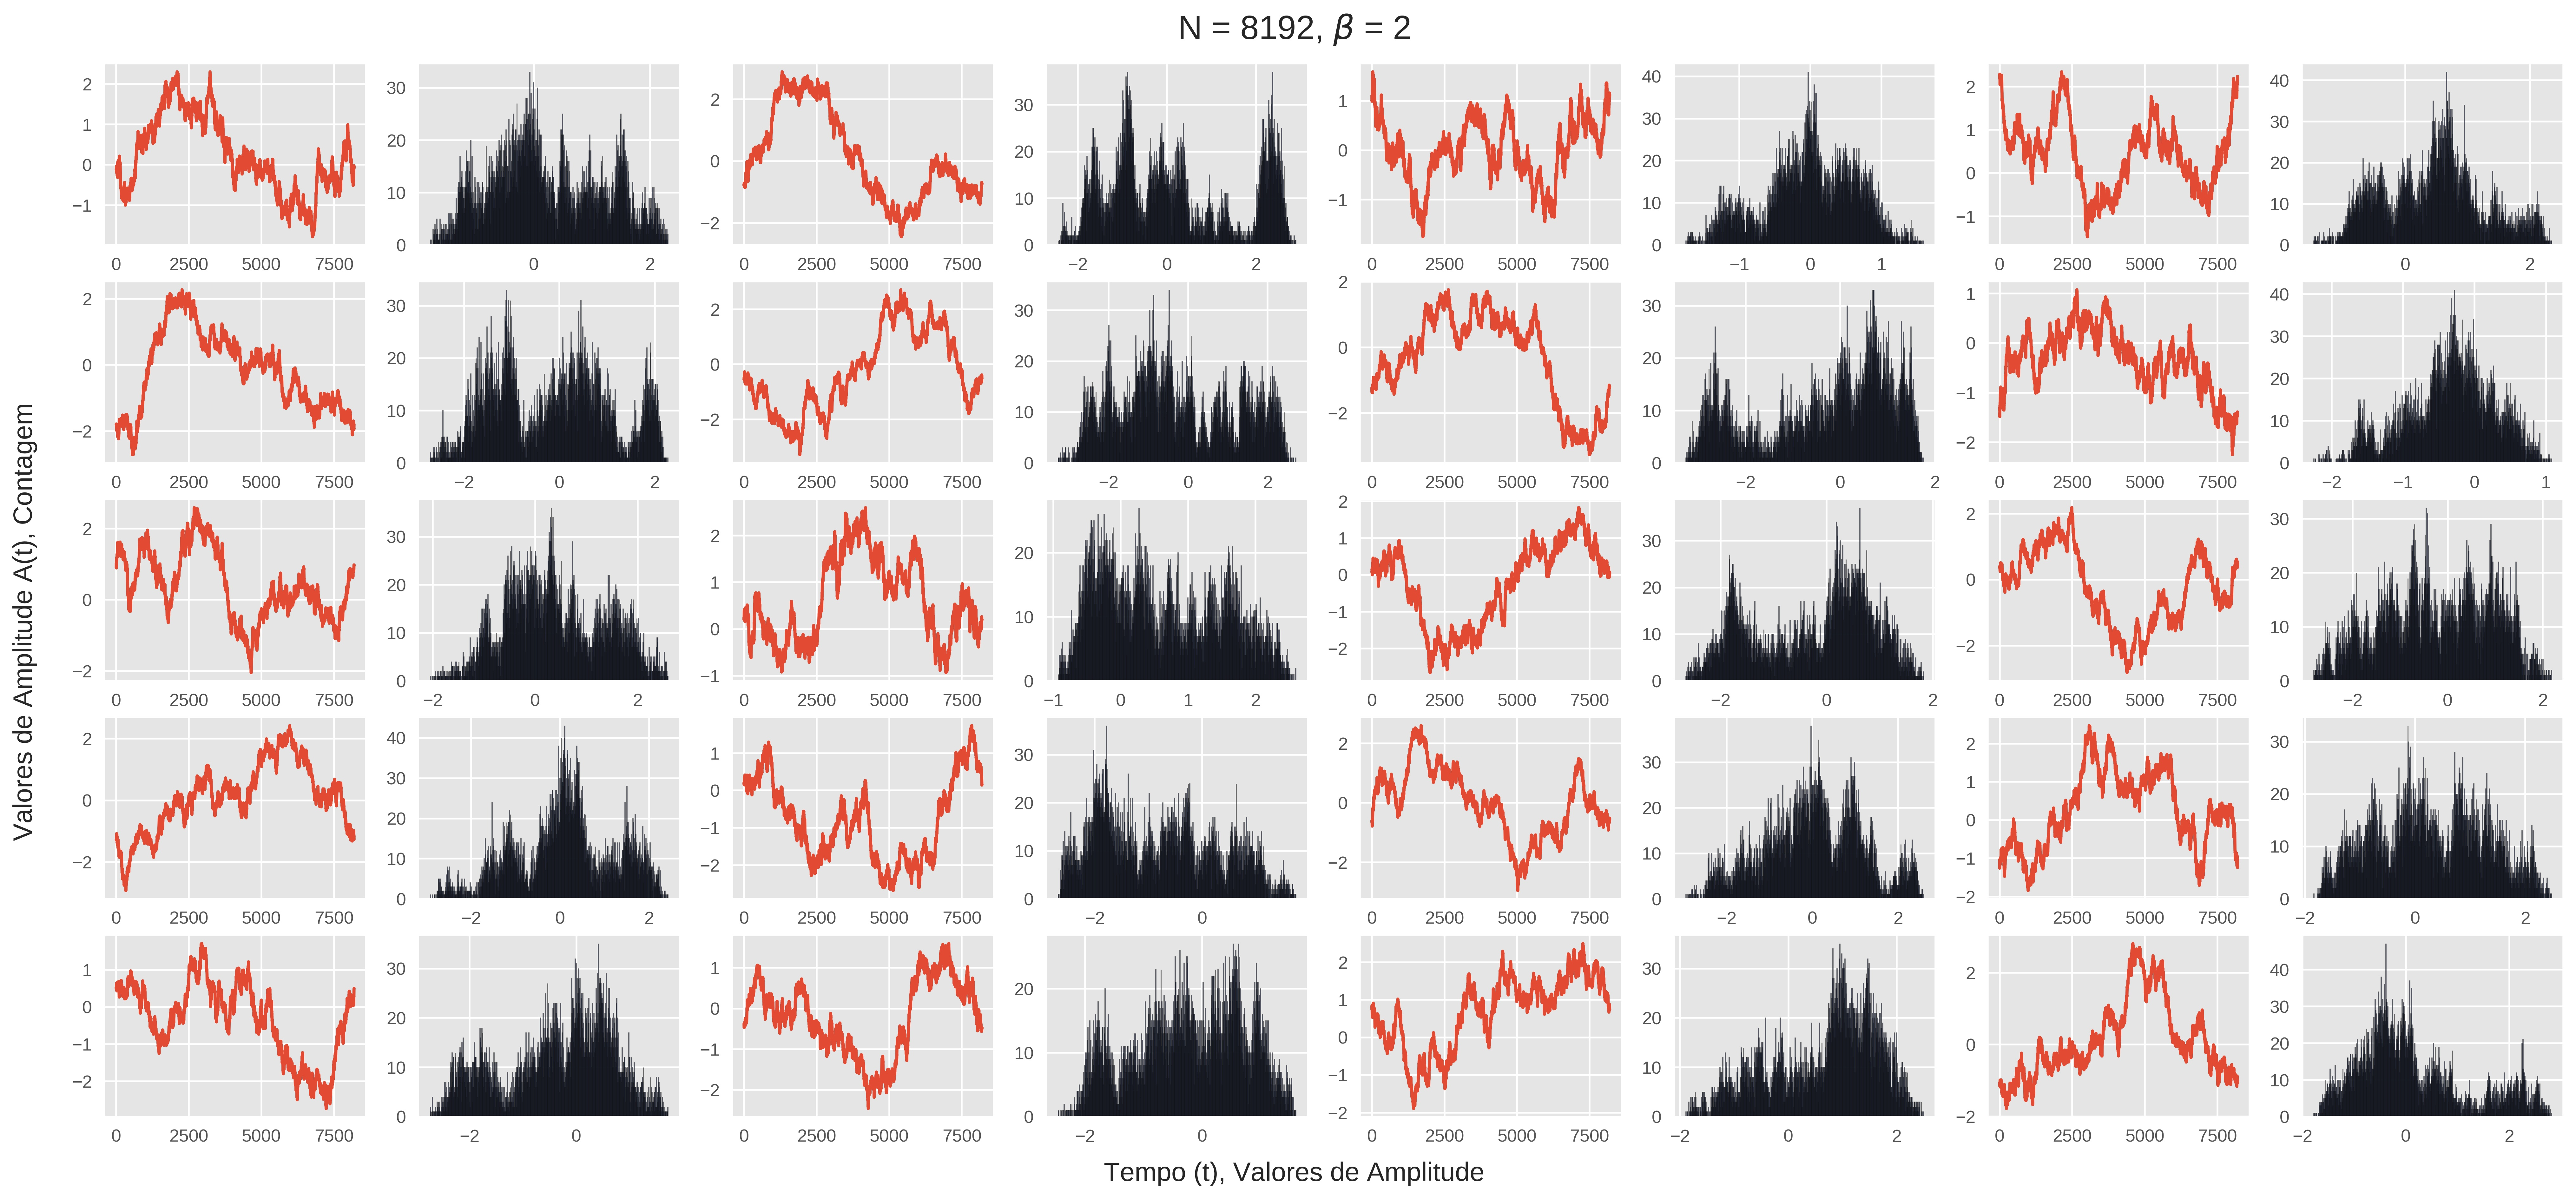
\includegraphics[scale=.35]{Figuras/ex2/Exercicio2_n_8192_beta_2.jpg}	%
  \end{adjustbox}
\end{figure}

%\begin{sidewaysfigure}[ht!]
	%\caption{Série e histogramas.}
	%\vspace{0mm}	% acrescentar o espaçamento vertical apropriado entre o título e a borda superior da figura
	%\begin{center}
%		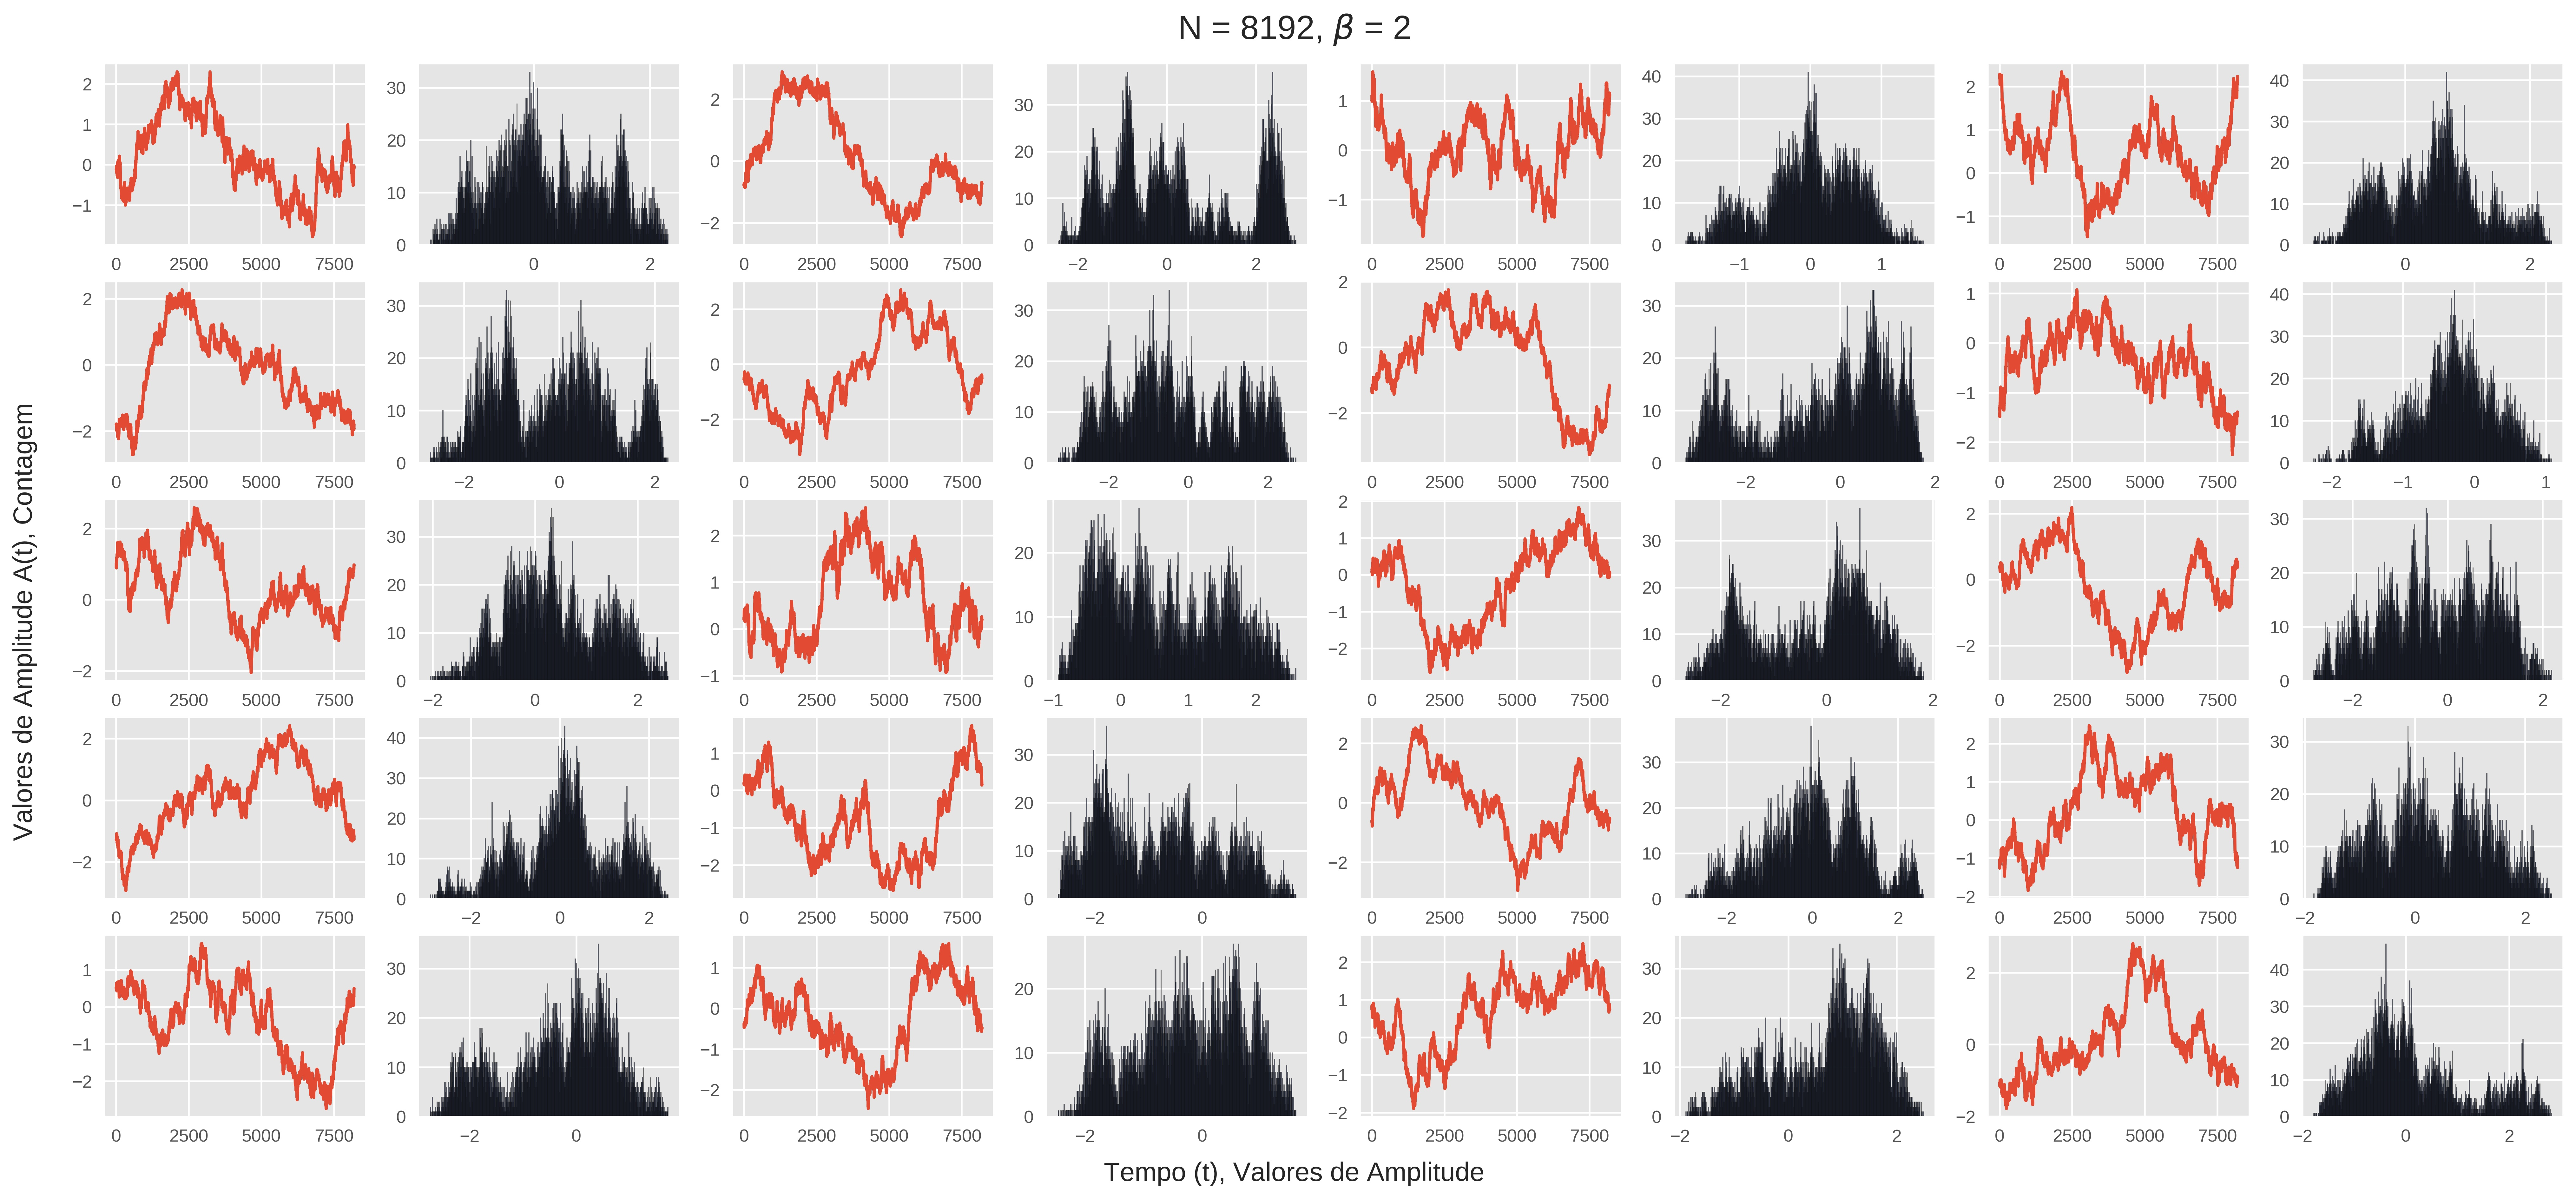
\includegraphics[scale=.3]{Figuras/ex2/Exercicio2_n_8192_beta_2.jpg}	
	%\end{center}
	%\vspace{-2mm}	% acrescentar o espaçamento vertical apropriado entre a borda inferior da figura e a legenda ou a fonte quando não há legenda (o valor pode ser negativo para subir)
%	\legenda{Figura 2.1:.}	% legenda - para deixar sem legenda usar comando \legenda{} (nunca deve-se comentar o comando \legenda)
%	\label{ex2_fig1}
	%\FONTE{}	% fonte consultada (elemento obrigatório, mesmo que seja produção do próprio autor)
%\end{sidewaysfigure}
\clearpage
Os mesmos arquivos .csv gerados na primeira questão foram também gerados para a família colornois: \textit{Exercicio2\_momentos.csv},  \textit{Exercicio2\_parametros.csv} e \textit{Exercicio2\_kmeans.csv}. Os resultados do agrupamento via kmeans são exibidos a seguir.

\begin{figure}[ht!]
	%\caption{Série e histogramas.}
	\vspace{0mm}	% acrescentar o espaçamento vertical apropriado entre o título e a borda superior da figura
	\begin{center}
		\resizebox{15cm}{!}{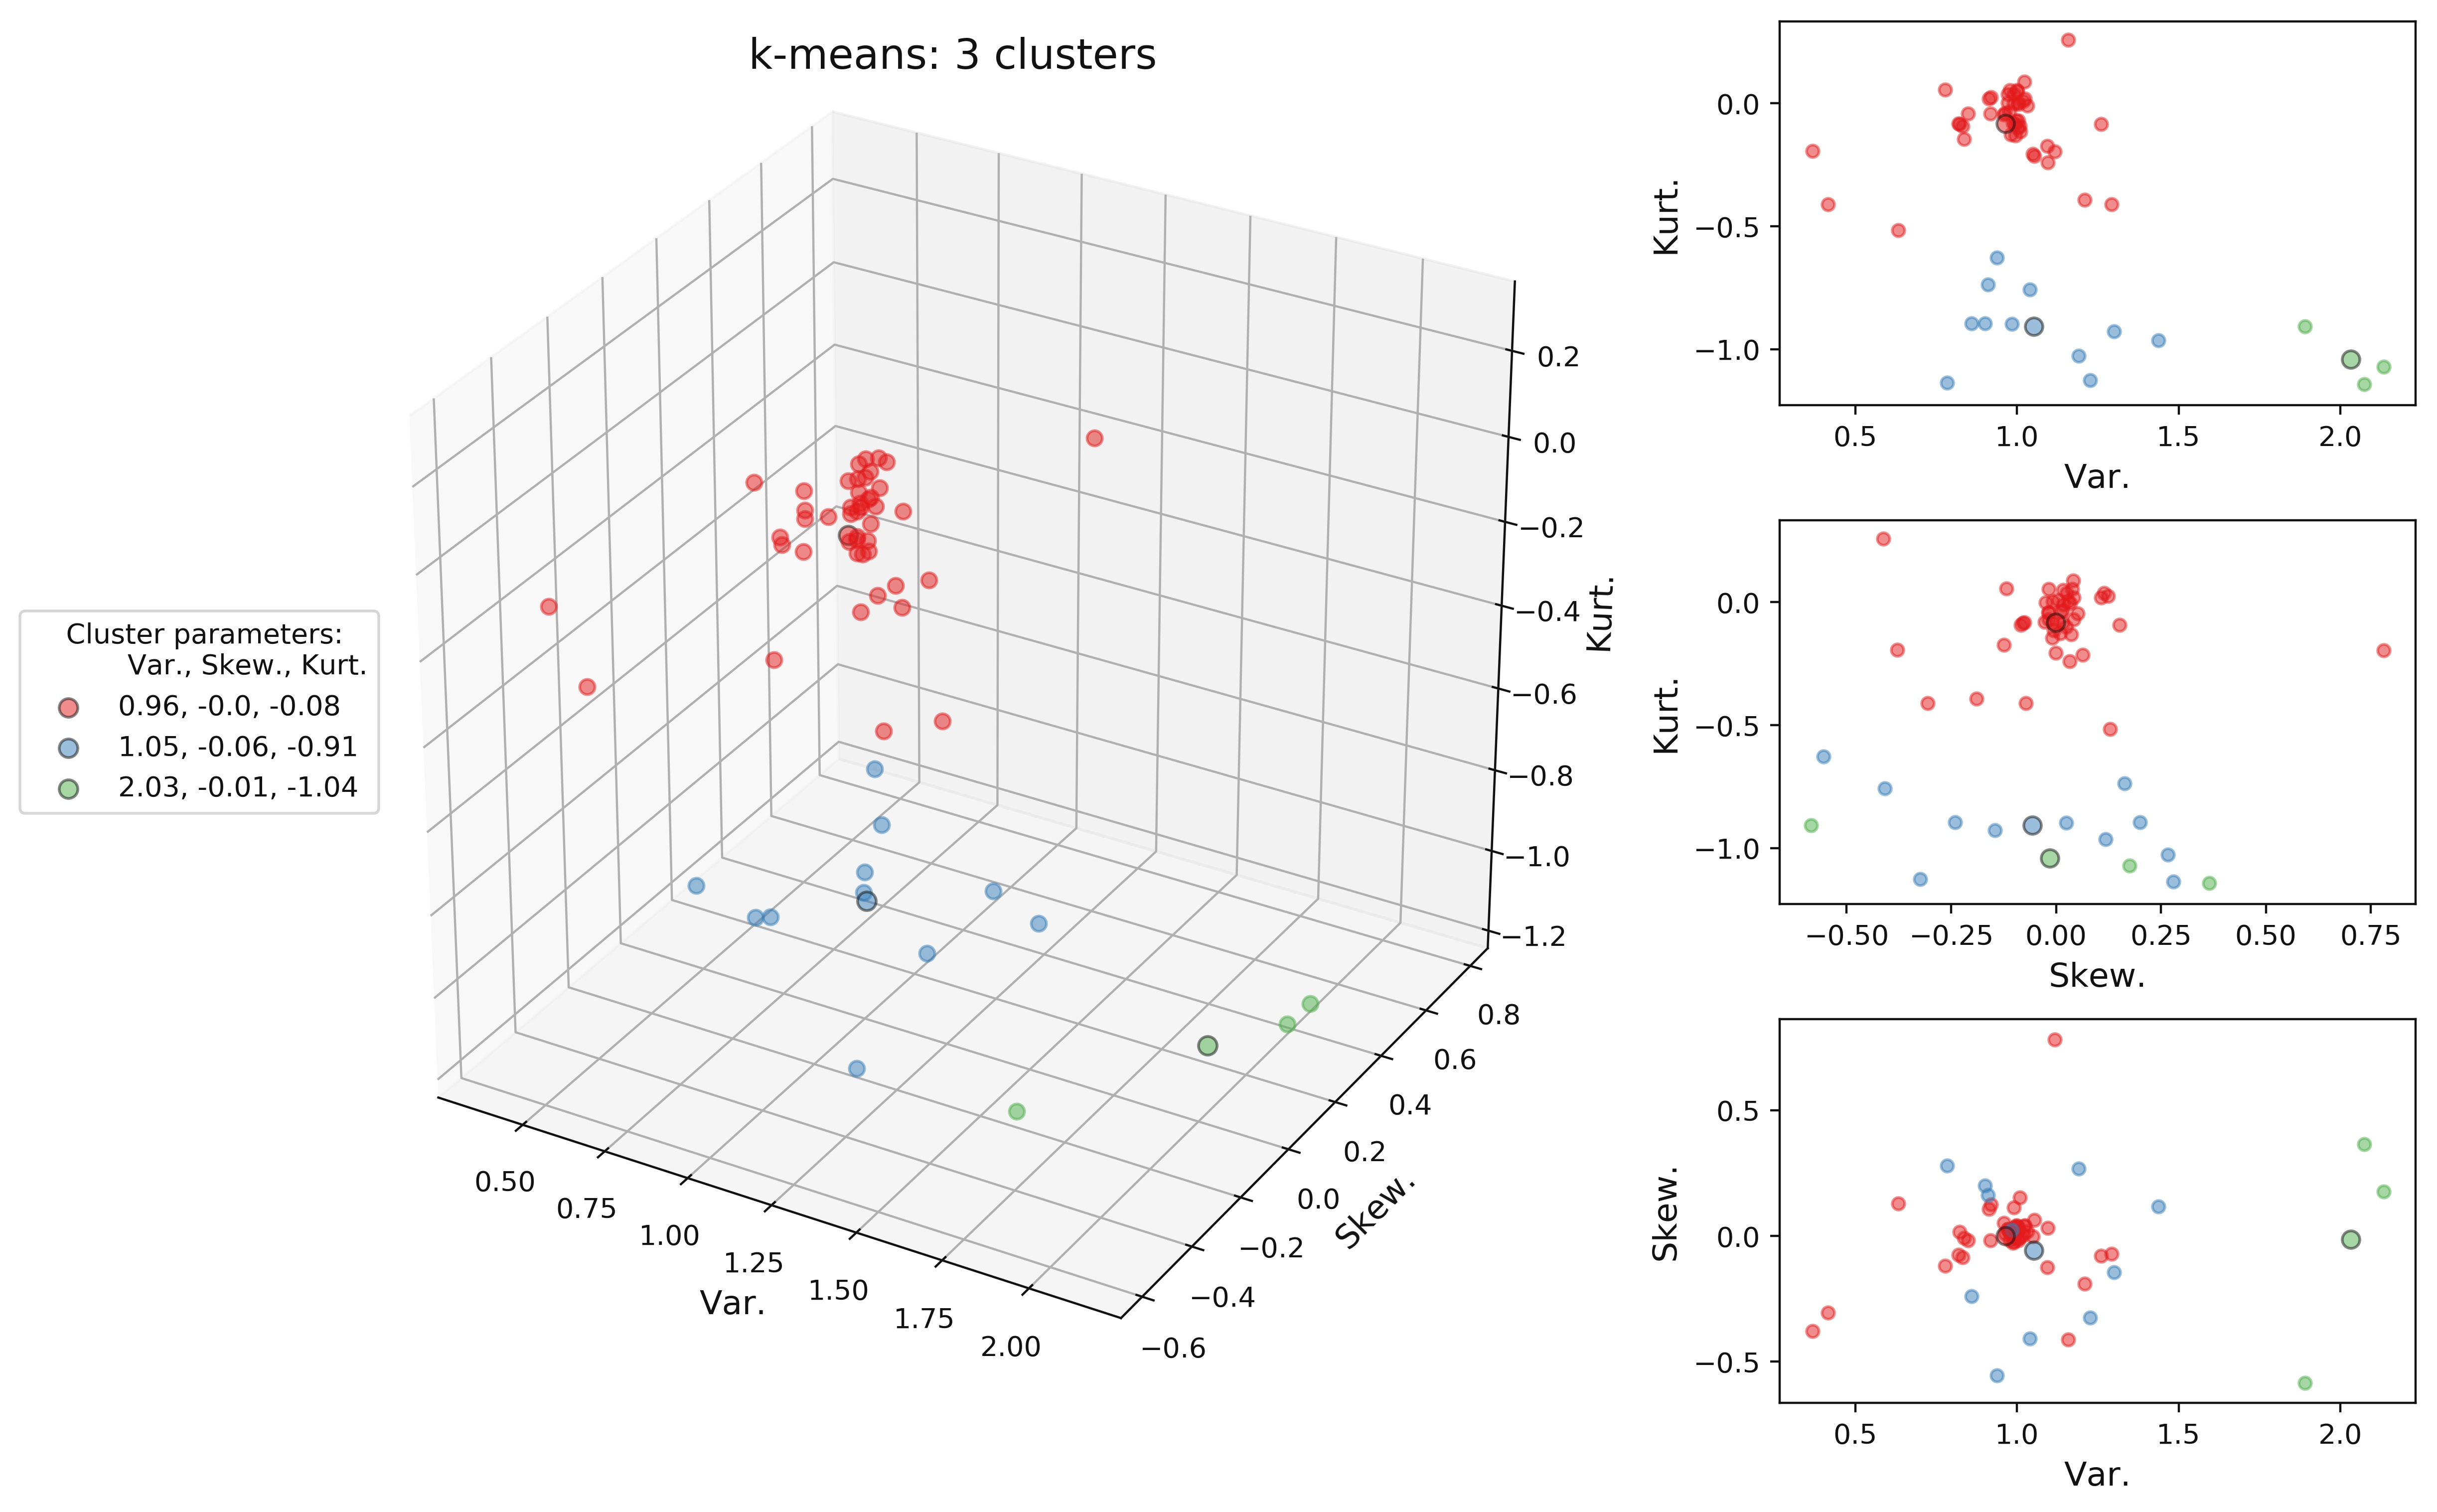
\includegraphics{Figuras/ex2/Exercicio2_cluster_3.jpg}}		
	\end{center}
	\vspace{-3mm}	% acrescentar o espaçamento vertical apropriado entre a borda inferior da figura e a legenda ou a fonte quando não há legenda (o valor pode ser negativo para subir)
	\legenda{Figura 2.2: Técnica kmeans no espaço de parâmetros variância x skewness x kurtosis para a família de sinais colornoise. Resultado para número de clusters $n\_c$ = 3.}	% legenda - para deixar sem legenda usar comando \legenda{} (nunca deve-se comentar o comando \legenda)
	\label{ex2_fig2}
	%\FONTE{}	% fonte consultada (elemento obrigatório, mesmo que seja produção do próprio autor)
\end{figure}

\begin{figure}[ht!]
	%\caption{Série e histogramas.}
	\vspace{0mm}	% acrescentar o espaçamento vertical apropriado entre o título e a borda superior da figura
	\begin{center}
		\resizebox{11cm}{!}{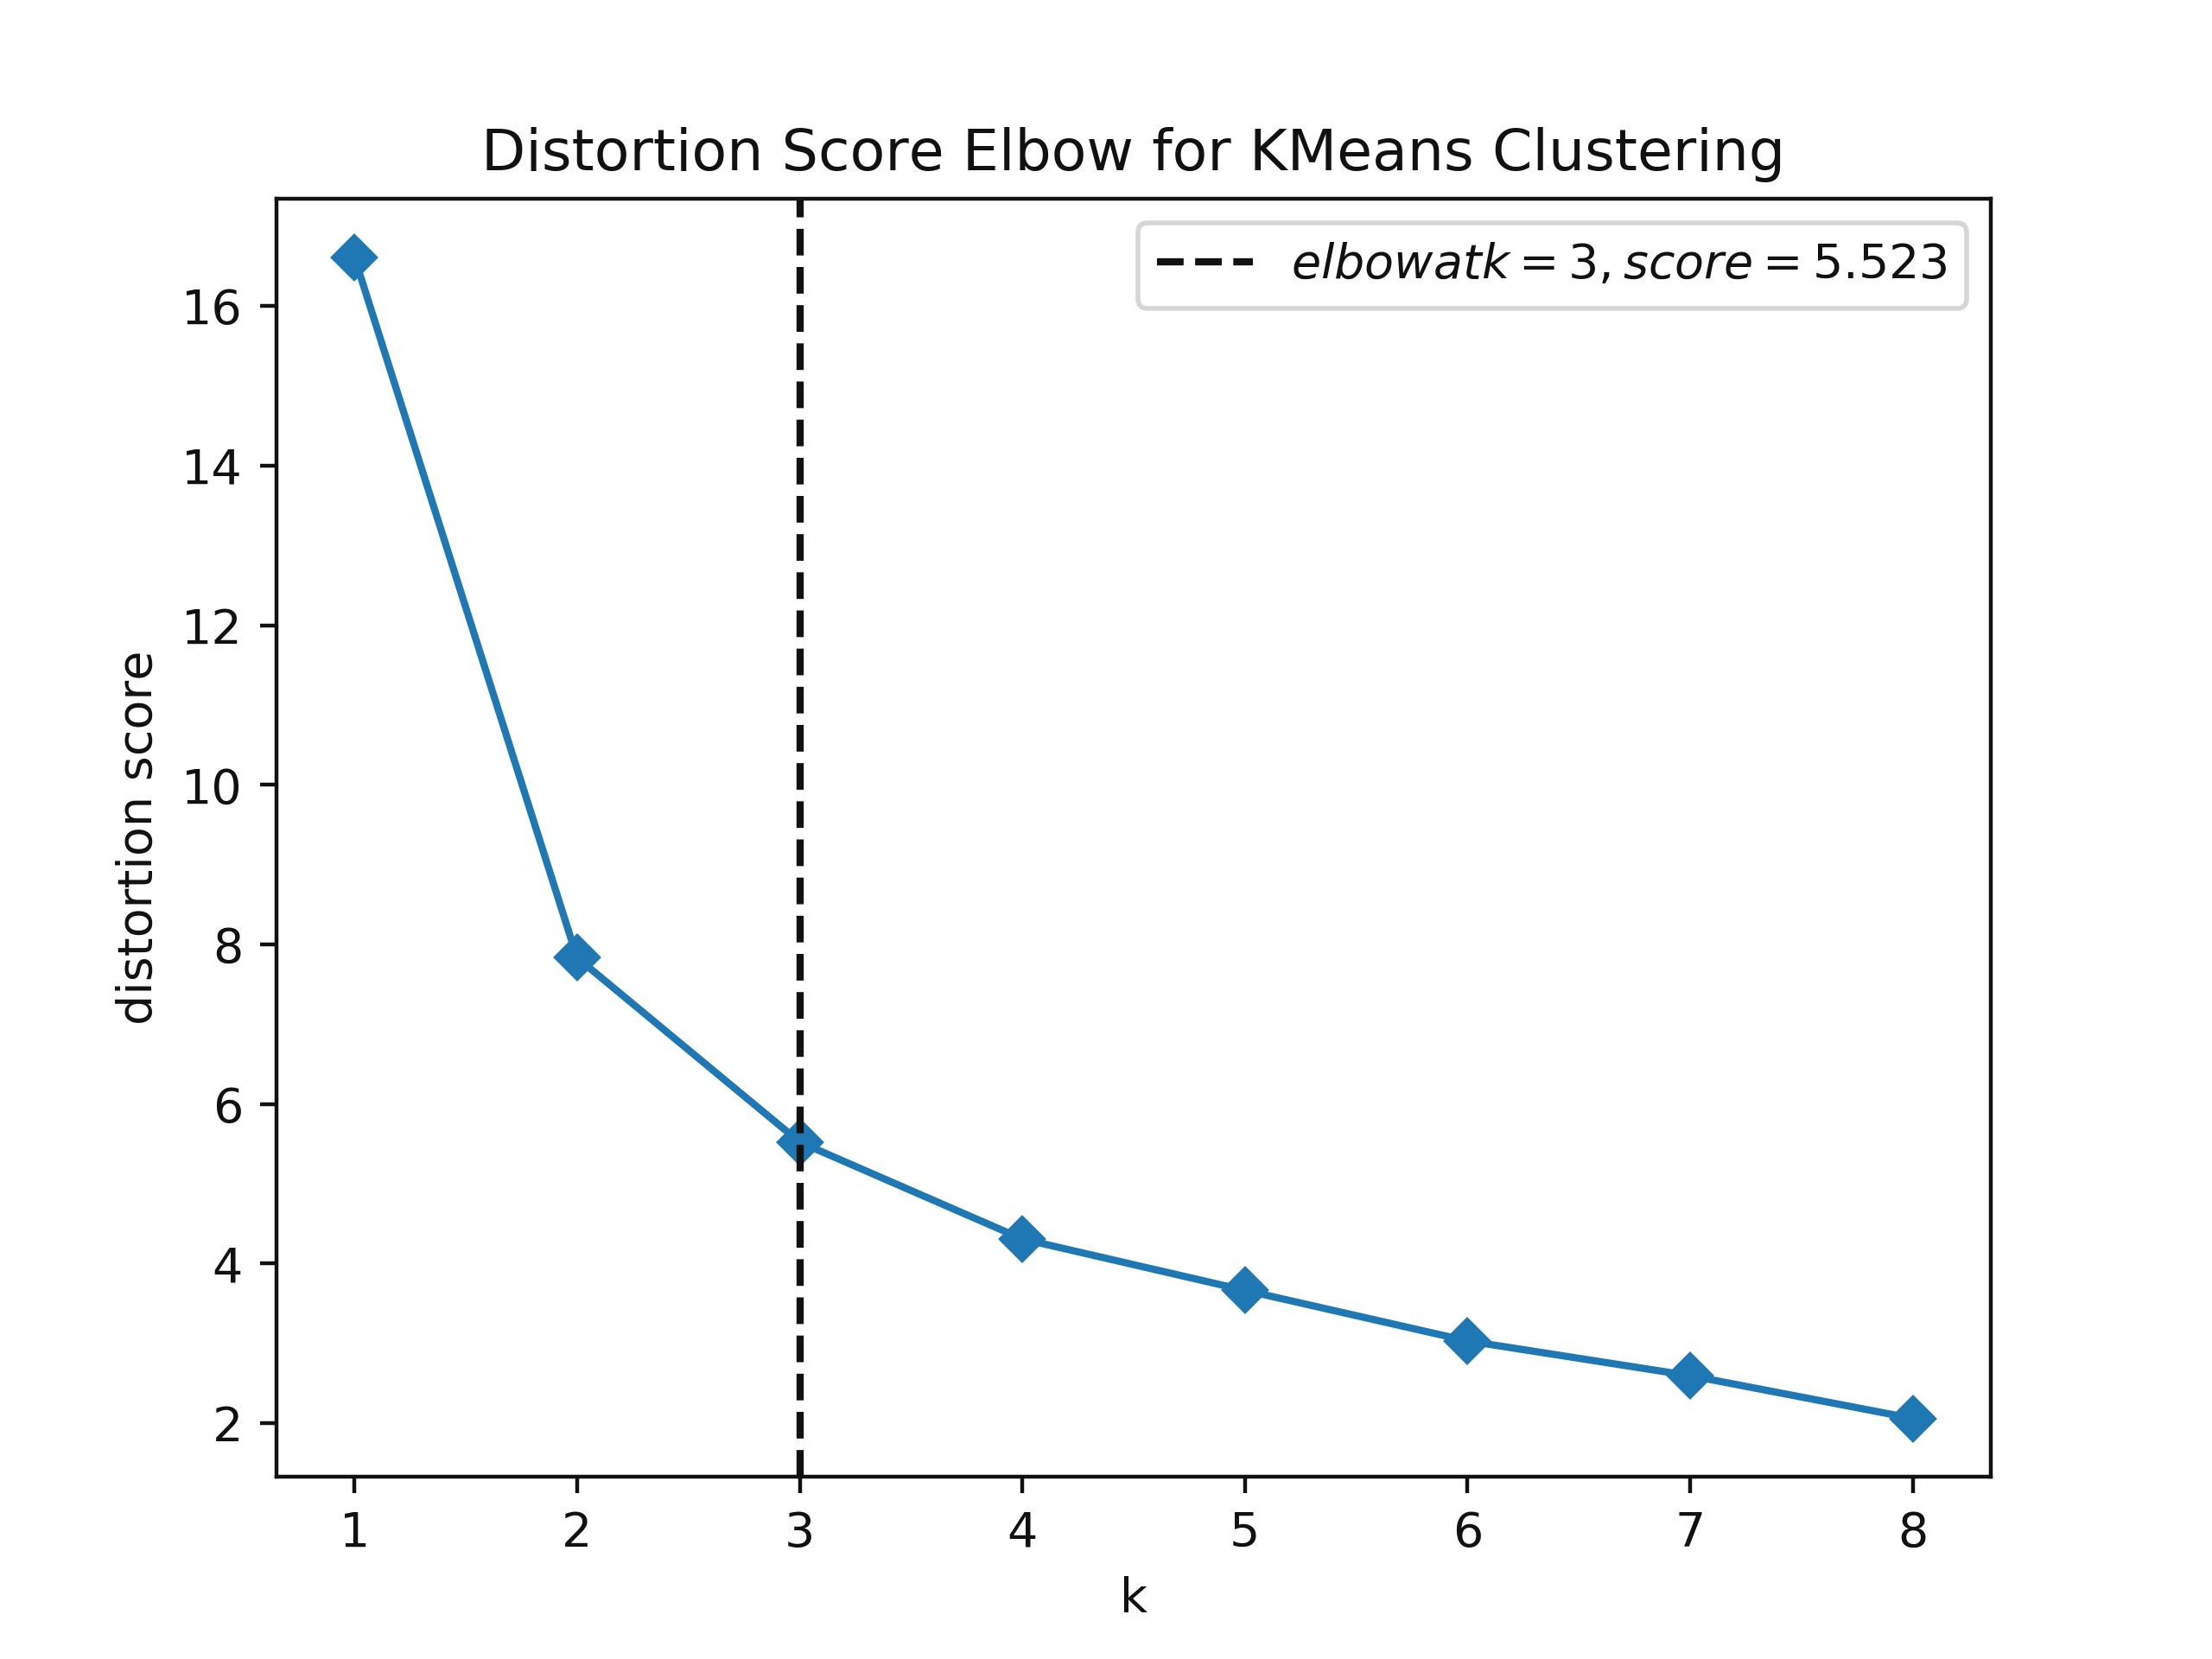
\includegraphics{Figuras/ex2/Exercicio2_elbow_algorithm.jpg}}		
	\end{center}
	\vspace{-3mm}	% acrescentar o espaçamento vertical apropriado entre a borda inferior da figura e a legenda ou a fonte quando não há legenda (o valor pode ser negativo para subir)
	\legenda{Figura 2.3: Resultado do método do cotovelo, mostrando que três clusters são necessários para agrupamento da família colornoise no espaço de parâmetros considerado.}	% legenda - para deixar sem legenda usar comando \legenda{} (nunca deve-se comentar o comando \legenda)
	\label{ex2_fig3}
	%\FONTE{}	% fonte consultada (elemento obrigatório, mesmo que seja produção do próprio autor)
\end{figure}